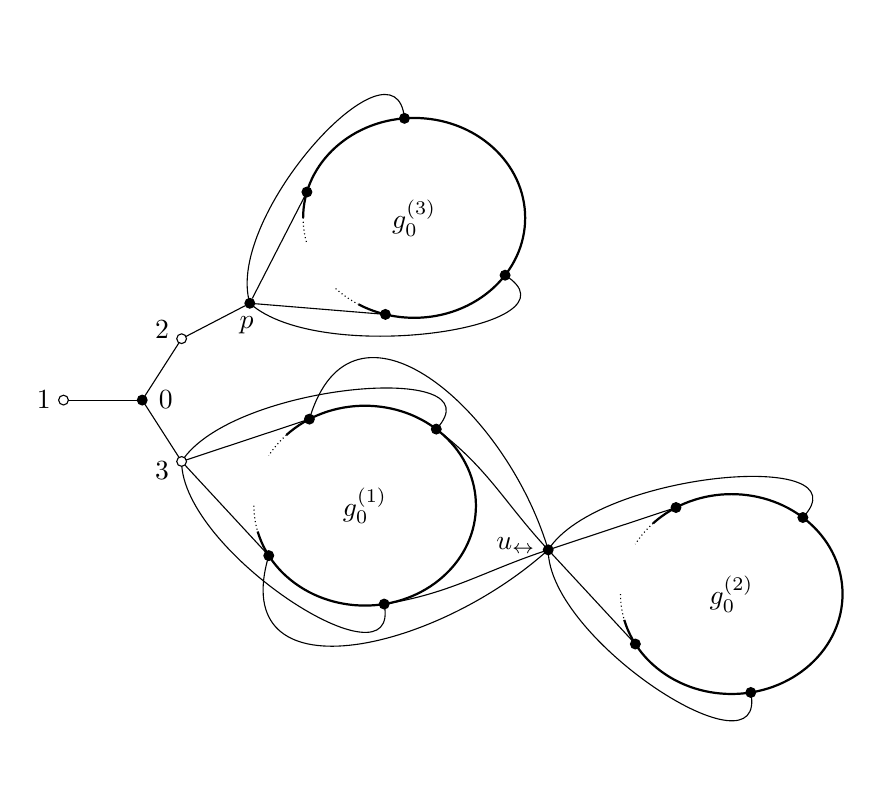
\begin{tikzpicture}[
  yscale = .9,
  label distance=-5.5pt,
  thin,
  vertex/.style={circle,draw=black,fill=black,inner sep=1.25pt,
    minimum size =0mm},
  attach/.style={circle,draw=black,fill=white,inner sep=1.25pt,
    minimum size =0mm},
  dots/.style={circle,fill=black,inner sep=.5pt,
    minimum size= 0pt}]

%%%%%%%%%%%%%%
% G^RT_\leftrightarrow graph
\begin{scope}[yshift=-.866 cm,xshift=.5cm,rotate=255,yshift = 2.41cm]

% Path and Labels    
  
  \node (v) at (0,2.41) [vertex] {};
  \node at (.05,2) {$u_\leftrightarrow$};
  
% Graphs

\foreach \j/\of in {1/0,2/4.82}{
\begin{scope}[yshift=\of cm]
  \foreach \i / \n /\t in {25 / n/ 15, 155 / 1/ 165, 225/ 2 / 120, 315 / {n-1}/60}{

    \node at (\i : 1.41) [vertex] {};
  }
  \node at (0,0) [rectangle,fill=white] {$g_0^{(\j)}$};
  
  \draw[thick] (240:1.41) arc (240:-60:1.41);
  \draw[densely dotted] (240:1.41)  arc (240:255:1.41);
  \draw[densely dotted] (285:1.41)  arc (285:300:1.41);
  
% Attaching Edges
  \foreach \i /\t in {25/15, 155/165}{
    \draw (\i:1.41) to[out=\i,in=\t] (0,-2.41);
  }
  
  \foreach \i \in in {225,315}{
    \draw (\i:1.41) to (0,-2.41);
  }
  
\end{scope}
}

  \draw (25:1.41) to [out = 115,in=-55] (0,2.41);
  \draw (155:1.41) to [out=65,in=-125] (0,2.41);
  \draw[looseness=1.5] (225:1.41) to [out=180,in=210] (0,2.41);
  \draw[looseness=1.5] (315:1.41) to [out=0,in=-30] (0,2.41);

\end{scope}

%%%%%%%%%%%%%%%%%%%%%%%%
% G^RT graph
\begin{scope}[xshift = .5 cm, yshift = .866 cm, rotate = -60, yshift = 3.41 cm]
% Path and Labels    
  
  \node (v) at (0,-2.41) [vertex]{};
  \node at (0.25,-2.6) {$p$};
  \draw (v) -- (0,-3.41); 
  
% Graph  
  \foreach \i / \n /\t in {25 / n/ 15, 155 / 1/ 165, 225/ 2 / 120, 315 / {n-1}/60}{

    \node at (\i : 1.41) [vertex] {};
  }
  \node at (0,0) [rectangle,fill=white] {$g_0^{(3)}$};
  
  \draw[thick] (240:1.41) arc (240:-60:1.41);
  \draw[densely dotted] (240:1.41)  arc (240:255:1.41);
  \draw[densely dotted] (285:1.41)  arc (285:300:1.41);

% Attaching Edges
  \foreach \i /\t in {25/15, 155/165}{
    \draw (\i:1.41) to [out=\i,in=\t] (0,-2.41);
  }
  
  \foreach \i \in in {225,315}{
    \draw (\i:1.41) to (v);
  }
  
\end{scope}

%%%%%%%
% Center stuff
\foreach \t in {60, 180, 300}{
  \draw (0,0) -- (\t:1);
}

\node (0) at (0,0) [vertex] {};
\node (1) at (180:1) [attach] {};
\node (2) at (60:1) [attach]{};
\node (3) at (-60:1) [attach]{};

\node at (0:.3) {$0$};
\node at (-1.25,0) {$1$};
\node at (.25,1) {$2$};
\node at (.25,-1) {$3$};
\end{tikzpicture}